%%% Uncomment for presentation mode
\documentclass[]{beamer}

%%% Uncomment for article mode
%\documentclass{article} 
%\usepackage{beamerarticle} 


\mode<presentation>
{
  \usetheme[]{Madrid}
  \useinnertheme{circles}
  \setbeamercovered{transparent=10}
  \setbeamertemplate{navigation symbols}{}
  \setbeamertemplate{frametitle continuation}[from second][\insertcontinuationtext]
}

\usepackage[english]{babel}
\usepackage[latin1]{inputenc}
\usepackage{times}
\usepackage[T1]{fontenc}
\usepackage{pgf}
\usepackage{color}
\usepackage{latexsym}
\usepackage[boxed,linesnumbered]{algorithm2e}
\usepackage{graphicx}
\usepackage{colortbl}

\usepackage{tikz}
\usetikzlibrary{arrows,decorations,backgrounds,matrix,automata,trees,shapes,shadows,plotmarks,calc,positioning}
\pgfdeclarelayer{background}
\pgfdeclarelayer{foreground}
\pgfsetlayers{background,main,foreground}

%\AtBeginSection[]
%{
%  \begin{frame}<beamer>{Outline}
%    \tableofcontents[currentsection]
%  \end{frame}
%}


%%%%%
\title[Learning BDI Plan Selection]{Learning Context Conditions for BDI Plan Selection}
\author[Singh et al.]{D.~Singh\inst{1} \and S.~Sardina\inst{1} \and L.~Padgham\inst{1} \and S.~Airiau\inst{2}}

\institute[RMIT \& UvA]{
\inst{1}School of Computer Science \& Information Technology\\RMIT University, Australia
\and
\inst{2}Institute for Logic, Language and Computation\\University of Amsterdam, The Netherlands
}

\date[AAMAS 2010]{Autonomous Agents and Multiagent Systems\\May 2010}
%%%%%


\begin{document}

\section{Presentation}

\begin{frame}[plain]
\setcounter{framenumber}{0}
\titlepage
\end{frame}

%
%\begin{frame}{Outline}
%\tableofcontents
%\end{frame}


%%%
\begin{frame}{Learning BDI Plan Selection}
\begin{center}
\resizebox{.7\paperwidth}{!}{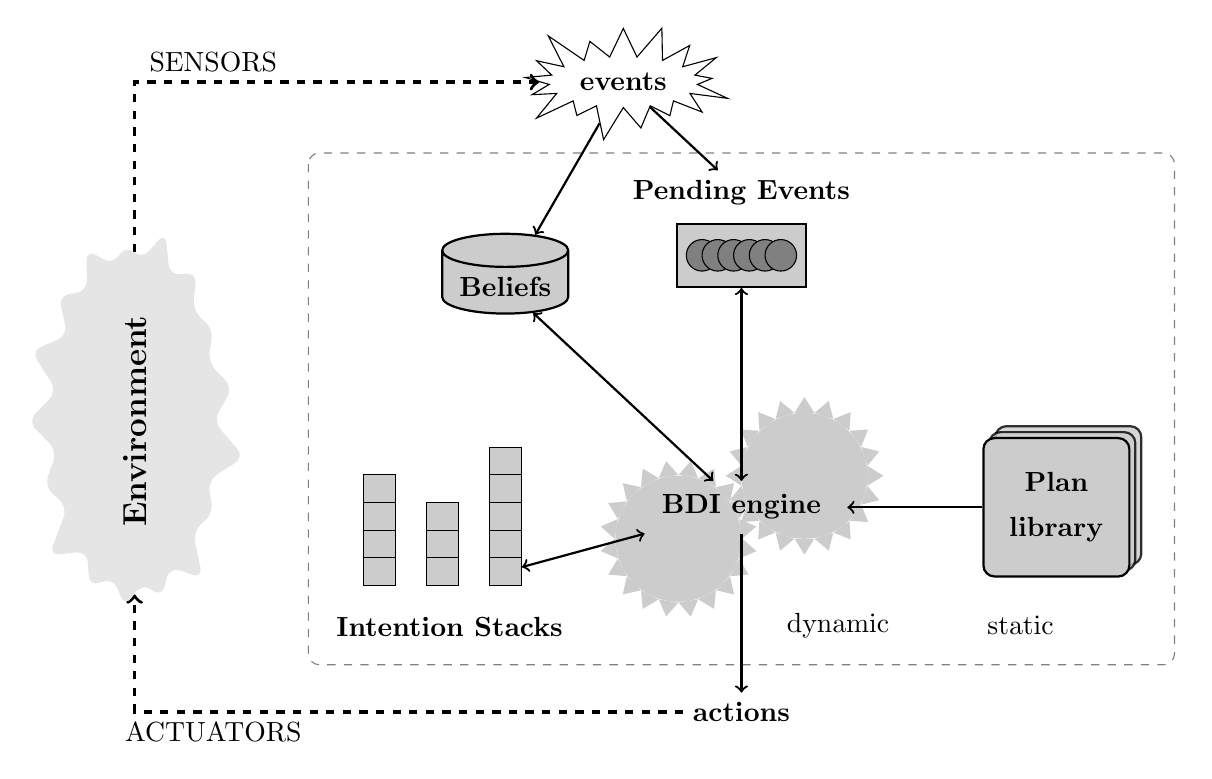
\begin{tikzpicture}

\tikzstyle{centityd}=[draw=black]
\tikzstyle{centityf}=[fill=black!20]
\tikzstyle{centity}=[centityd,centityf]
\tikzstyle{entity}=[centity,thick,text centered,anchor=center]


\node[anchor=east] at (6,4.5)  {dynamic};
\node[anchor=west] at (7,4.5) {static};


\node (database) at (1,8.8)  (B)
	[cylinder,entity,shape border rotate=90,minimum width=1.6cm,shape aspect=.3]
	{\textbf{Beliefs}};


\node  (environment)  
       [below left of=B, rounded corners, minimum height=3cm,
       starburst,fill=black!10,rotate=90,shift={(-1cm,4cm)}] 
       {\textbf{\large Environment}};



\node at (4,10) (eventQueue) {{\bf Pending Events}};
\begin{pgfonlayer}{foreground}
\foreach \x in {3.5,3.7,...,4.5}
\draw [fill=black!50](\x,9.2) circle (0.2);
\end{pgfonlayer}
%\path (4,9.1) node (Q) {}; 
\draw (4,9.2) node (Q) 
	[entity, text width=1.4cm, minimum height=0.8cm] {};




\foreach \x in {4,3,2,1}
\draw (-.6,5) node (I) [anchor=south,draw, centity, text width=.5em,
	minimum height=\x em]{};
\foreach \x in {3,2,1}
\draw (0.2,5) node (I) [anchor=south,draw,centity, text width=.5em,
	minimum height=\x em]{};
\foreach \x in {5,4,3,2,1}
\draw (1,5) node (I) [anchor=south,draw, centity, text width=0.5em,
	minimum height=\x em]{};
\node[below left of=I] (Intentions) {{\bf  Intention Stacks}};


% { [start chain=1]
% % \node [on chain,draw] at (0,6) {};
%     \foreach \x in {1,2,...,11} {
%        \x, \node [draw,on chain=1] {};
%     }
% }

\begin{pgfonlayer}{foreground}
\node[anchor=center] at (4,6)  (deli) 
	{\begin{tabular}{c}
     	\textbf{BDI engine} 
     \end{tabular}};
\node at (4,3.4) (actions) {{\bf actions}};
\node at (2.5,11.4) [starburst,centityd] (in) {{\bf events}};


\draw node (P) 
	[right of=deli,xshift=3cm,rounded corners, double copy
	shadow={opacity=0.8},text centered, entity, minimum height=5em] 
	{	\begin{tabular}{c} 
          \textbf{Plan} \\[1ex]
          \textbf{library}
         \end{tabular}	};



\draw[thick,->] (in) -- (B) ; 
\draw[thick,->] (in) -- (eventQueue) ; 
\draw[thick,->] (deli) -- (actions) ; 
\draw[thick,<->] (deli) -- (I) ; 
\draw[thick,<->] (deli) -- (B) ; 
\draw[thick,<-] (deli) -- (P) ;
\draw[thick,<->] (deli) -- (Q) ; 
\end{pgfonlayer}








\begin{pgfonlayer}{background}

%% Dotted box encapuslating the agent
\path (-1.5,10.5) node (c) {};
\path (9.5,4) node (d) {};
\path[fill=none,rounded corners, draw=black!50, dashed] (c) rectangle (d);




\draw[->,very thick,dashed] (environment) 
		|- node[above,xshift=1cm] {SENSORS}
	 	(in);
\draw[->,very thick,dashed] (actions.west) 
		-| node[below,xshift=1cm] {ACTUATORS}
		(environment.west);
\end{pgfonlayer}


\foreach \x in {-9,9,...,360}
\fill [rotate around={\x:(3.2,5.6)},centityf] 
	(4.0,5.4743) -- (4.2 ,5.6) -- (4.0,5.7257) -- (4.0,5.3487);
\fill [centityf] (3.2,5.6) circle (0.8);

\foreach \x in {0,18,...,360}
\fill [rotate around={\x:(4.8,6.4)},centityf] 
	(5.6,6.2743)-- (5.8,6.4) -- (5.6,6.5257) -- (5.6,6.2743);
\fill [centityf] (4.8,6.4) circle (0.8);


\end{tikzpicture}}\\
Plan \alert{$\delta$} is a strategy to resolve event \alert{$e$} whenever context \alert{$\psi$} holds.\\ Our focus is the \alert{plan selection problem} i.e. to learn \alert{$\psi$}.
\end{center}
\end{frame}

%%%
\begin{frame}{Motivation for Learning}
\onslide+<+->
\begin{block}{The Belief-Desire-Intention (BDI) model of agency}
\begin{itemize}
\item<+-> Is robust and well suited for dynamic environments.
\item<+-> Has inspired several development platforms \\(PRS, AgentSpeak(L), JACK, JASON, SPARK, 3APL and others).
\item<+-> Has been deployed in practical systems like UAVs.
\end{itemize}
\end{block}
\onslide+<+->
\begin{block}{Nonetheless}
\begin{itemize}
\item<+-> Behaviours (plans) and the situations where they apply (context) are \alert{fixed at design time}.
\item<+-> For complex domain, it is difficult to specify \alert{complete} context conditions upfront.
\item<+-> Once deployed, the agent has no means to \alert{adapt} to changes in the initial environment.
\end{itemize}
\end{block}
\end{frame}

%%%
\begin{frame}{Learning From Plan Choices}
\begin{center}
\only<1>{\resizebox{.7\paperwidth}{!}{%!TEX root = ../dsingh-aamas10.tex
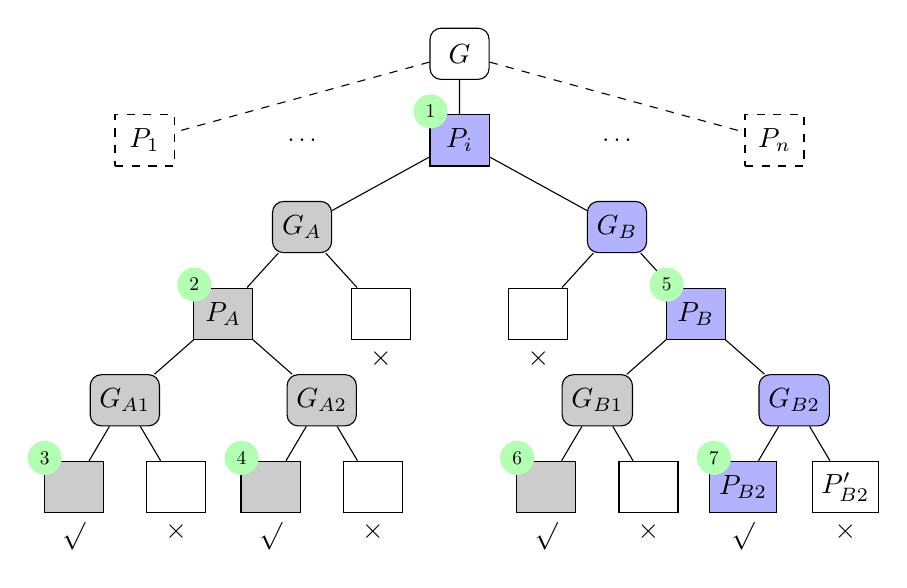
\begin{tikzpicture}[level distance=1.1cm]
\tikzstyle{txt}=[scale=.9]
\tikzstyle{succ}=[label=below:$\surd$]
\tikzstyle{fail}=[label=below:$\times$]
\tikzstyle{trace}=[solid,style=circle,fill=green!30,above left=0.3cm,scale=.7]

\tikzstyle{planbox}=[draw,minimum height=0.65cm,minimum width=0.75cm]
\tikzstyle{planbox2}=[planbox,fill=blue!30]
\tikzstyle{planbox3}=[planbox,fill=black!20]
\tikzstyle{goalbox}=[draw,rounded corners,minimum height=0.65cm,minimum width=0.75cm]
\tikzstyle{goalbox2}=[goalbox,fill=blue!30]
\tikzstyle{goalbox3}=[goalbox,fill=black!20]

	
\tikzstyle{level 1}=[sibling distance=4.0cm] 
\tikzstyle{level 2}=[sibling distance=4cm] 
\tikzstyle{level 3}=[sibling distance=2cm]
\tikzstyle{level 4}=[sibling distance=2.5cm]
\tikzstyle{level 5}=[sibling distance=1.3cm]

\node[goalbox,yshift=1cm,solid] (T) {$G$}
	child[dashed] {node[planbox] (P1) {$P_1$}}
	child[solid] {node[planbox2] (Pi) {$P_i$}
		child {node[goalbox3] {$G_A$}
			child {node[planbox3] {$P_{A}$}
				child {node[goalbox3] {$G_{A1}$}
					child {node[planbox3,succ] {$\phantom{P}$}
						node[trace]{$3$}
					}
					child {node[planbox,fail] {$\phantom{P}$} 
					edge from parent node[txt,right,near start] {}
					}
				}
				child {node[goalbox3] {$G_{A2}$}
					child {node[planbox3,succ] {$\phantom{P}$}
						node[trace]{$4$}
					}
					child {node[planbox,fail] {$\phantom{P}$} 
						edge from parent node[txt,right,near start] {}
					}
				}
				node[trace]{$2$}
			}
			child {node[planbox,fail] {$\phantom{P}$} 
				edge from parent node[txt,right,near start] {}
			}
		}
		child {node[goalbox2] {$G_{B}$}
			child {node[planbox,fail] {$\phantom{P}$}
				edge from parent node[txt,left,near start] {}
			}
			child {node[planbox2] {$P_B$}
				child {node[goalbox3] {$G_{B1}$}
					child {node[planbox3,succ] {$\phantom{P}$}
						node[trace]{$6$}
					}
					child {node[planbox,fail] {$\phantom{P}$}
						edge from parent node[txt,right,near start] {}
					}
				}
				child {node[goalbox2] {$G_{B2}$}
					child {node[planbox2,succ] {$P_{B2}$}
						node[trace]{$7$}
					}
					child {node[planbox,fail] {$P_{B2}'$}
						edge from parent node[txt,right,near start] {}
					}
				}
			node[trace]{$5$}
			}
		}
		node[trace]{$1$}
	}
	child[dashed] {node[planbox] (Pn) {$P_n$}}
;
\node[txt] at ($ (P1)!.5!(Pi) $) {$\ldots$};
\node[txt] at ($ (Pi)!.5!(Pn) $) {$\ldots$};

\end{tikzpicture}
}\\
Execution trace for successful resolution of goal $G$ given world state $w$. Success means that all correct choices were made.}
\only<2>{\resizebox{.7\paperwidth}{!}{%!TEX root = ../dsingh-aamas10.tex
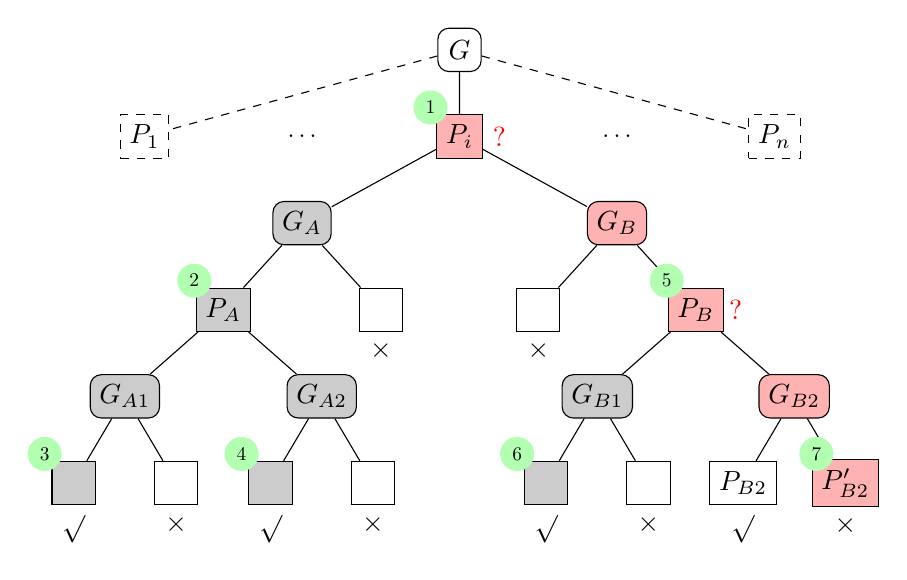
\begin{tikzpicture}[level distance=1.1cm]
\tikzstyle{txt}=[scale=.9]
\tikzstyle{succ}=[label=below:$\surd$]
\tikzstyle{fail}=[label=below:$\times$]
\tikzstyle{trace}=[solid,style=circle,fill=green!30,above left=0.3cm,scale=.7]

\tikzstyle{planbox}=[draw,minimum height=0.55cm,minimum width=0.55cm]
\tikzstyle{planbox2}=[planbox,fill=black!20]
\tikzstyle{planbox3}=[planbox,fill=red!30]
\tikzstyle{goalbox}=[draw,rounded corners,minimum height=0.55cm,minimum width=0.55cm]
\tikzstyle{goalbox2}=[goalbox,fill= black!20]
\tikzstyle{goalbox3}=[goalbox,fill=red!30]

	
\tikzstyle{level 1}=[sibling distance=4.0cm] 
\tikzstyle{level 2}=[sibling distance=4cm] 
\tikzstyle{level 3}=[sibling distance=2cm]
\tikzstyle{level 4}=[sibling distance=2.5cm]
\tikzstyle{level 5}=[sibling distance=1.3cm]

\node[goalbox,yshift=1cm,solid] (T) {$G$}
	child[dashed] {node[planbox] (P1) {$P_1$}}
	child[solid] {node[planbox3] (Pi) {$P_i$}
		child {node[goalbox2] {$G_A$}
			child {node[planbox2] {$P_{A}$}
				child {node[goalbox2] {$G_{A1}$}
					child {node[planbox2,succ] {$\phantom{P}$}
						node[trace]{$3$}
					}
					child {node[planbox,fail] {$\phantom{P}$} 
					edge from parent node[txt,right,near start] {}
					}
				}
				child {node[goalbox2] {$G_{A2}$}
					child {node[planbox2,succ] {$\phantom{P}$}
						node[trace]{$4$}
					}
					child {node[planbox,fail] {$\phantom{P}$} 
						edge from parent node[txt,right,near start] {}
					}
				}
				node[trace]{$2$}
			}
			child {node[planbox,fail] {$\phantom{P}$} 
				edge from parent node[txt,right,near start] {}
			}
		}
		child {node[goalbox3] {$G_{B}$}
			child {node[planbox,fail] {$\phantom{P}$}
				edge from parent node[txt,left,near start] {}
			}
			child {node[planbox3] (PB) {$P_B$}
				child {node[goalbox2] {$G_{B1}$}
					child {node[planbox2,succ] {$\phantom{P}$}
						node[trace]{$6$}
					}
					child {node[planbox,fail] {$\phantom{P}$}
						edge from parent node[txt,right,near start] {}
					}
				}
				child {node[goalbox3] {$G_{B2}$}
					child {node[planbox,succ] {$P_{B2}$}}
					child {node[planbox3,fail] {$P_{B2}'$}
						node[trace]{$7$}
						edge from parent node[txt,right,near start] {}
					}
				}
				node[trace]{$5$}
				node[red,right=0.3cm]{?}
			}
		}
		node[trace]{$1$}
		node[red,right=0.3cm]{?}
	}
	child[dashed] {node[planbox] (Pn) {$P_n$}}
;
\node[txt] at ($ (P1)!.5!(Pi) $) {$\ldots$};
\node[txt] at ($ (Pi)!.5!(Pn) $) {$\ldots$};

\end{tikzpicture}
}\\
Possible execution trace where goal $G$ is not resolved for $w$.\\ Should non-leaf plans consider this failure meaningful?}
\end{center}
\note{
The figure shows an example BDI plan library represented as a tree. Here plans nodes are suffixed with the label $P$ and goals with $G$. The parent of a plan is the goal type it was designed to handle. The children are sub-goals that must succeed in a sequential manner in order for the plan to succeed. Leaf plans interact directly with the environment by performing actions that may succeed (ticks) or fail (crosses) for a given world state. 

Here the successful resolution of the top-level goal $G$ requires 4 sequential actions to be performed.}
\end{frame}

%%%
\begin{frame}{BDI Learning Framework}
\onslide+<+->
\begin{block}{Previous work (Airiau~et~al. 2009)}
\begin{itemize}
\item<+-> Augment static logical context conditions of plans with dynamic \alert{decision trees}.
\item<+-> Select plans \alert{probabilistically} based on their ongoing expectation of success.
\item<+-> \alert{Learn context conditions} over time by training decision trees using success/failure outcomes under various situations.
\end{itemize}
\end{block}
\onslide+<+->
\begin{block}{Contributions of this paper}
\begin{itemize}
\item<+-> A more principled analysis of the work in [Airiau~et~al. 2009].
\item<+-> Learning with \alert{plan applicability} (using thresholds to filter plans that do not apply in a given situation).
\end{itemize}
\end{block}
\note{In tradition BDI, applicability is determined by whether the propositional context condition holds or not (boolean). A similar account using our framework then could be taken using a threshold. Plans with expectations of success below this threshold would thereby be considered not applicable.}
\end{frame}

%%%
\begin{frame}{Learning Considerations}
\onslide+<+->
\begin{block}{Collecting training data (building DTs)}
\begin{itemize}
\item<+-> \alert{ACL}: Aggressive approach that considers all failures as meaningful.
\item<+-> \alert{BUL}: Conservative approach that records failures selectively when choices were well-informed.
\item<+-> Success is always recorded for both approaches.
\end{itemize}
\end{block}
\onslide+<+->
\begin{block}{Improving plan selection (using DTs)}
\begin{itemize}
\item<+-> Obtain a numeric measure of \alert{confidence} in the ongoing decision tree classification.
\item<+-> Use the confidence measure to \alert{adjust selection weights} during probabilistic plan selection. 
\end{itemize}
\end{block}
\note{This gives us four configurations. Aggressive or conservative sampling with or without the confidence measure. However we do not present an account of the conservative recording scheme with the coverage measure since the stability notion in effect implies full coverage.}
\end{frame}

%%%
\begin{frame}{Assumptions}
\begin{block}{}
We explore how best to learn under an \alert{imposed goal-plan hierarchy} in an idealised setting.
\end{block}
\onslide+<+->
\begin{block}{}
\begin{itemize}
\item<+-> Recursive/parameterised events or relational beliefsets not addressed.
\item<+-> BDI failure recovery mechanism disabled during learning.
\item<+-> Synthetic plan library with empty initial context conditions used.
\item<+-> Simple account of non-determinism: successful actions have a $10\%$ probability of failure.
\end{itemize}
\end{block}
\onslide+<+->
\begin{block}{}
Ongoing work aims to relax these constraints towards a more practical system.
\end{block}


\end{frame}

%%%
\begin{frame}[allowframebreaks]{Results: Does Selective Recording Matter?}

\centering\resizebox{.7\paperwidth}{!}{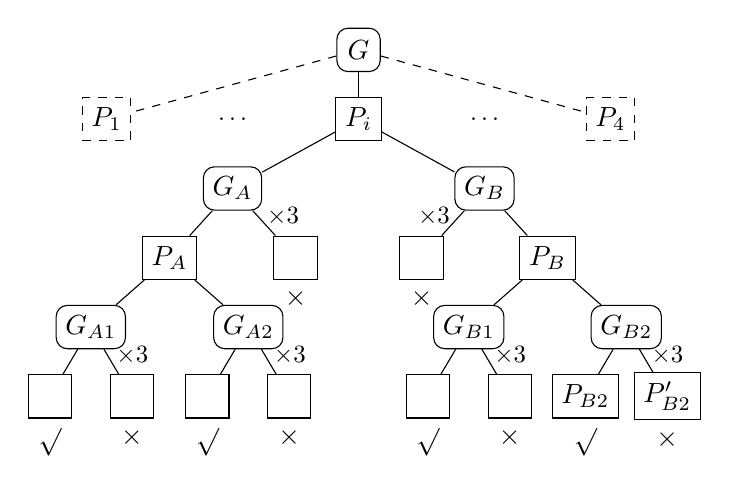
\begin{tikzpicture}[scale=0.8,level distance=1.1cm]
\tikzstyle{txt}=[scale=.9]
\tikzstyle{succ}=[label=below:$\surd$]
\tikzstyle{fail}=[label=below:$\times$]

\tikzstyle{planbox}=[draw,minimum height=0.55cm,minimum width=0.55cm]
\tikzstyle{goalbox}=[draw,rounded corners,minimum height=0.55cm,minimum width=0.55cm]

	
\tikzstyle{level 1}=[sibling distance=4.0cm] 
\tikzstyle{level 2}=[sibling distance=4cm] 
\tikzstyle{level 3}=[sibling distance=2cm]
\tikzstyle{level 4}=[sibling distance=2.5cm]
\tikzstyle{level 5}=[sibling distance=1.3cm]

\node[goalbox,yshift=1cm,solid] (T) {$G$}
	child[dashed] {node[planbox] (P1) {$P_1$}}
	child[solid] {node[planbox] (Pi) {$P_i$}
		child {node[goalbox] {$G_A$}
			child {node[planbox] {$P_{A}$}
				child {node[goalbox] {$G_{A1}$}
					child {node[planbox,succ] {$\phantom{P}$}}
					child {node[planbox,fail] {$\phantom{P}$} 
					edge from parent node[txt,right,near start] {$\times 3$}
					}
				}
				child {node[goalbox] {$G_{A2}$}
					child {node[planbox,succ] {$\phantom{P}$}}
					child {node[planbox,fail] {$\phantom{P}$} 
						edge from parent node[txt,right,near start] {$\times 3$}
					}
				}
			}
			child {node[planbox,fail] {$\phantom{P}$} 
				edge from parent node[txt,right,near start] {$\times 3$}
			}
		}
		child {node[goalbox] {$G_{B}$}
			child {node[planbox,fail] {$\phantom{P}$}
				edge from parent node[txt,left,near start] {$\times 3$}
			}
			child {node[planbox] {$P_B$}
				child {node[goalbox] {$G_{B1}$}
					child {node[planbox,succ] {$\phantom{P}$}}
					child {node[planbox,fail] {$\phantom{P}$}
						edge from parent node[txt,right,near start] {$\times 3$}
					}
				}
				child {node[goalbox] {$G_{B2}$}
					child {node[planbox,succ] {$P_{B2}$}}
					child {node[planbox,fail] {$P_{B2}'$}
						edge from parent node[txt,right,near start] {$\times 3$}
					}
				}
			}
		}
	}
	child[dashed] {node[planbox] (P4) {$P_4$}}
;
\node[txt] at ($ (P1)!.5!(Pi) $) {$\ldots$};
\node[txt] at ($ (Pi)!.5!(P4) $) {$\ldots$};

\end{tikzpicture}
}

Structure where both schemes show \alert{comparable performance}.

\centering\resizebox{.7\paperwidth}{!}{%!TEX root = ../dsingh-aamas10-poster.tex
\begin{tikzpicture}[x=0.0032cm,y=9cm]
    % Draw the axes and grid lines
    \draw[-] (0,0) -- (0,1) -- (5000,1) -- (5000,0) -- cycle; 
    \draw[-,thin, dotted, ystep=0.2, xstep=5000] (0,0) grid (5000,1);
    \foreach \x in {1000, 2500, 4000}  \draw [-,xshift=0](\x,4pt) -- (\x,-1pt);
    \foreach \y in {0.0,0.2,0.4,0.6,0.8,1.0}  \draw [-,yshift=0](4pt,\y) -- (-1pt,\y);
    \foreach \x/\xtext in {1000/1000, 2500/2500, 4000/4000} \node at (\x,0) [below] {\xtext};
    \foreach \y/\ytext in {0.0,0.2,0.4,0.6,0.8,1.0}  \node at (0,\y) [left] {\ytext};
    \node at (0,1.15) {Success};
    \node at (4150,0.1) {Iterations};
    \draw[-,red] plot[mark=x,mark size=10,mark options={color=red}] 
			file {figs/data/testImpactvars2.CP.tikzdata};
    \draw[-,blue] plot[mark=o,mark size=6,mark options={color=blue}] 
			file {figs/data/testImpactvars2.SP.tikzdata};
    % Also draw the expected convergence: 0.9^4 actions=0.6561
    \draw[dashed,-,yshift=0](0,0.6561) -- (5000,0.6561);
	\node at (5700,0.5) {$\mathcal{T}3$};

\end{tikzpicture}
}

Performance of ACL (crosses) vs. BUL (circles). \\Dashed line shows optimal performance.

\end{frame}

%%%
\begin{frame}{Results: Learning with Applicability Filtering}

\onslide+<+->

\begin{block}{}
Plan execution is generally not cost-free, so agent may fail a goal \alert{without even trying} if it is unlikely to succeed.
\end{block}
\onslide+<+->

\centering\resizebox{.7\paperwidth}{!}{%!TEX root = ../dsingh-aamas10.tex
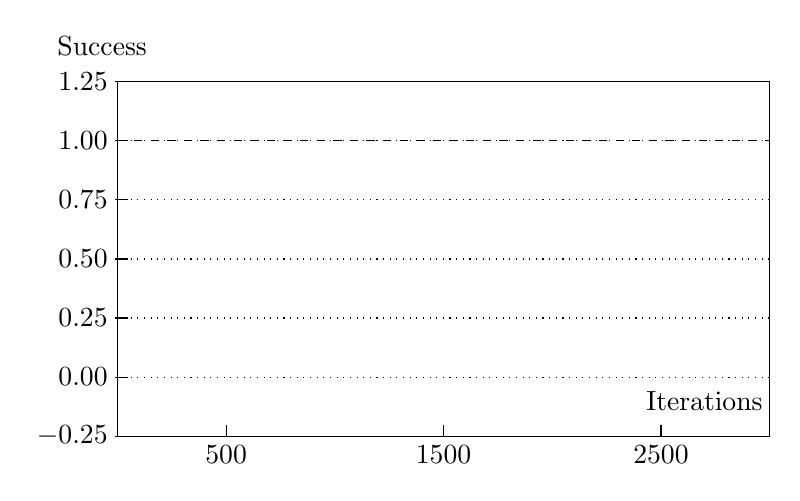
\begin{tikzpicture}[x=0.00276cm,y=3cm]
    % Draw the axes and grid lines
    \draw[-] (0,-0.25) -- (0,1.25) -- (3000,1.25) -- (3000,-0.25) -- cycle; 
    \draw[-,thin, dotted, ystep=0.25, xstep=3000] (0,-0.25) grid (3000,1.25);
    \foreach \x in {500, 1500, 2500}  \draw [-,xshift=0,yshift=-0.25](\x,-0.20) -- (\x,-0.25);
    \foreach \y in {-0.25,0.00,0.25,0.50,0.75,1.00,1.25}  \draw [-,yshift=0](4pt,\y) -- (-1pt,\y);
    \foreach \x/\xtext in {500/500, 1500/1500, 2500/2500} \node at (\x,-0.25) [below] {$\xtext$};
    \foreach \y/\ytext in {-0.25,0.00,0.25,0.50,0.75,1.00,1.25}  \node at (0,\y) [left] {$\ytext$};
    \node at (-70,1.4) {Success};
    \node at (2700,-0.1) {Iterations};
    \draw[-,red] plot[mark=x,mark size=4,mark options={color=red}] 
			file {figs/data/test05v3gmt.CP.tikzdata};
    \draw[-,blue] plot[mark=o,mark size=2,mark options={color=blue}] 
			file {figs/data/test05v3gmt.SP.tikzdata};
    % Also draw the expected convergence: 0.9^8 actions=0.43046
    \draw[dashed,-,yshift=0](0,1.0) -- (3000,1.0);

\end{tikzpicture}
}

Performance of ACL (crosses) vs. BUL (circles). \\Dashed line shows optimal performance.

\end{frame}

%%%
\begin{frame}[allowframebreaks]{Improving Plan Selection}

\onslide+<+->
\begin{block}{Coverage-based confidence measure}
Idea is that confidence in a plan's decision tree increases as more choices below the plan are \alert{covered}.
\end{block}

\centering\resizebox{.6\paperwidth}{!}{%!TEX root = ../dsingh-aamas10.tex
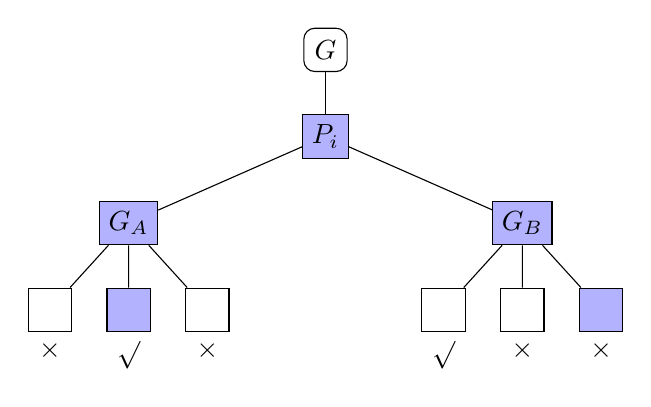
\begin{tikzpicture}[level distance=1.1cm]
\tikzstyle{txt}=[scale=.9]
\tikzstyle{succ}=[label=below:$\surd$]
\tikzstyle{fail}=[label=below:$\times$]

\tikzstyle{planbox}=[draw,minimum height=0.55cm,minimum width=0.55cm]
\tikzstyle{planbox2}=[planbox,fill=blue!30]
\tikzstyle{goalbox}=[draw,rounded corners,minimum height=0.55cm,minimum width=0.55cm]
\tikzstyle{goalbox2}=[planbox,fill=blue!30]

\tikzstyle{level 1}=[sibling distance=4.0cm] 
\tikzstyle{level 2}=[sibling distance=5cm] 
\tikzstyle{level 3}=[sibling distance=1cm]
\tikzstyle{level 4}=[sibling distance=2.5cm]
\tikzstyle{level 5}=[sibling distance=1.3cm]

\node[goalbox,yshift=1cm,solid] (T) {$G$}
	child[solid] {node[planbox2] (Pi) {$P_i$}
		child {node[goalbox2] {$G_A$}
			child {node[planbox,fail] {$\phantom{P}$}} 
			child {node[planbox2,succ] {$\phantom{P}$}} 
			child {node[planbox,fail] {$\phantom{P}$}} 
		}
		child {node[goalbox2] {$G_{B}$}
			child {node[planbox,succ] {$\phantom{P}$}} 
			child {node[planbox,fail] {$\phantom{P}$}} 
			child {node[planbox2,fail] {$\phantom{P}$}} 
		}
	}
;

\end{tikzpicture}
}

Highlighted path shows $1/9$ possible choices under $P_i$.

\begin{block}{How confidence influences plan selection}
\begin{itemize}
\item When the plan has not been tried before (zero coverage) we bias towards the default weight of $0.5$.
\item As more options are tried (approaching full coverage), we progressively bias towards the decision tree probability $p_T(w)$.
\end{itemize}
\end{block}
\begin{block}{Plan selection weight calculation}
\begin{equation*}
\Omega'_T(w) = 0.5 + \left[  c_T(w) *  \left( p_T(w) - 0.5 \right)  \right].
\end{equation*}
\end{block}
\end{frame}

%%%
\begin{frame}[allowframebreaks]{Results: Goal-Plan Hierarchy B}

\centering\resizebox{.7\paperwidth}{!}{%!TEX root = ../dsingh-aamas10-poster.tex
\begin{tikzpicture}[x= 0.00533cm,y=9cm]
	\definecolor{darkblue}{rgb}{0.1,0.1,0.5}
	\definecolor{darkred}{rgb}{0.8,0.0,0.1}
    % Draw the axes and grid lines
    \draw[-] (0,0) -- (0,1) -- (3000,1) -- (3000,0) -- cycle; 
    \draw[-,thin, dotted, ystep=0.2, xstep=3000] (0,0) grid (3000,1);
    \foreach \x in {500, 1500, 2500}  \draw [-,xshift=0](\x,4pt) -- (\x,-1pt);
    \foreach \y in {0.0,0.2,0.4,0.6,0.8,1.0}  \draw [-,yshift=0](4pt,\y) -- (-1pt,\y);
    \foreach \x/\xtext in {500/500, 1500/1500, 2500/2500} \node at (\x,0) [below] {\xtext};
    \foreach \y/\ytext in {0.0,0.2,0.4,0.6,0.8,1.0}  \node at (0,\y) [left] {\ytext};
    \node at (0,1.15) {Success};
    \node at (2500,0.1) {Iterations};
    \draw[-,darkred] plot[mark=x,mark size=10,mark options={color=darkred}] 
			file {figs/data/test05v3gm.CC.tikzdata};
    \draw[-,thin, densely dashed,black] plot[mark=x,mark size=10,mark options={color=black}] 
			file {figs/data/test05v3gm.CP.tikzdata};
    \draw[-,darkblue] plot[mark=o,mark size=6,mark options={color=darkblue}] 
			file {figs/data/test05v3gm.SP.tikzdata};
    % Also draw the expected convergence: 0.9^8 actions=0.43046
    \draw[dashed,-,yshift=0](0,0.43046) -- (3000,0.43046);
	\node at (3450,0.5) {$\mathcal{T}2$};

\end{tikzpicture}
}

Performance of ACL+$\Omega'_T$ (red crosses) vs. previous results\\ in structure that suits the conservative \alert{BUL} approach. Dashed line shows optimal performance.

\end{frame}

%%%
\begin{frame}[allowframebreaks]{Results: Learning with Applicability Filtering}

\centering\resizebox{.7\paperwidth}{!}{%!TEX root = ../dsingh-aamas10-poster.tex
\begin{tikzpicture}[x=0.00533cm,y=6cm]
    % Draw the axes and grid lines
    \draw[-] (0,-0.25) -- (0,1.25) -- (3000,1.25) -- (3000,-0.25) -- cycle; 
    \draw[-,thin, dotted, ystep=0.25, xstep=3000] (0,-0.25) grid (3000,1.25);
    \foreach \x in {500, 1500, 2500}  \draw [-,xshift=0,yshift=-0.25](\x,-0.20) -- (\x,-0.25);
    \foreach \y in {-0.25,0.00,0.25,0.50,0.75,1.00,1.25}  \draw [-,yshift=0](4pt,\y) -- (-1pt,\y);
    \foreach \x/\xtext in {500/500, 1500/1500, 2500/2500} \node at (\x,-0.25) [below] {\xtext};
    \foreach \y/\ytext in {0.00,0.25,0.50,0.75,1.00}  \node at (0,\y) [left] {\ytext};
    \node at (-70,1.45) {Success};
    \node at (2500,-0.1) {Iterations};
    \draw[-,red] plot[mark=x,mark size=4,mark options={color=red}] 
			file {figs/data/test05v3gmt.CC.tikzdata};
    \draw[-,thin,densely dashed,black] plot[mark=x,mark size=4,mark options={color=black}] 
			file {figs/data/test05v3gmt.CP.tikzdata};
    \draw[-,thin,densely dashed,black] plot[mark=o,mark size=2,mark options={color=black}] 
			file {figs/data/test05v3gmt.SP.tikzdata};
    % Also draw the expected convergence: 0.9^8 actions=0.43046
    \draw[dashed,-,yshift=0](0,1.0) -- (3000,1.0);
	\node at (3500,0.5) {$\mathcal{T}2,20\%$};

\end{tikzpicture}
}

Performance of ACL+$\Omega'_T$ (red crosses) vs. previous results

\end{frame}

%%%
\begin{frame}{Learning Context Conditions for BDI Plan Selection}
\begin{itemize}
\item<+-> Learning BDI plan selection is desirable since designing exact \alert{context conditions} for practical systems is non-trivial.
\end{itemize}
\begin{itemize}
\item<+-> Our approach uses decision trees to learn the context condition of plans.
\end{itemize}
\begin{itemize}
\item<+-> We suggest that an \alert{aggressive sampling scheme} combined with a \alert{coverage-based confidence measure} is a good candidate approach for the general hierarchical setting.
\end{itemize}
\end{frame}

%%%--SECTION
\newcounter{finalframe}
\setcounter{finalframe}{\value{framenumber}}
\appendix

%%%
\begin{frame}
\setcounter{framenumber}{\value{finalframe}}
  \frametitle<presentation>{References}
  \begin{thebibliography}{10}
  \beamertemplatearticlebibitems
  \bibitem{Bratman88}
	M.~Bratman, D.~Israel, and M.~Pollack.
	\newblock Plans and resource-bounded practical reasoning.
	\newblock {\em Computational Intelligence}, 4(4):349--355, 1988.
  \bibitem{Rao96}
    A.S.~Rao
	\newblock AgentSpeak (L): BDI agents speak out in a logical computable language.
	\newblock {\em Lecture Notes in Computer Science}, 1038:42--55, 1996.
  \bibitem{Airiau:IJAT09}
	S.~Airiau, L.~Padgham, S.~Sardina, and S.~Sen.
	\newblock Enhancing Adaptation in {BDI} Agents Using Learning Techniques.
	\newblock {\em International Journal of Agent Technologies and Systems}, 2009.
  \end{thebibliography}
\end{frame}

%%%
\begin{frame}{Goal-Plan Structure T1}
\setcounter{framenumber}{\value{finalframe}}

\centering\resizebox{.7\paperwidth}{!}{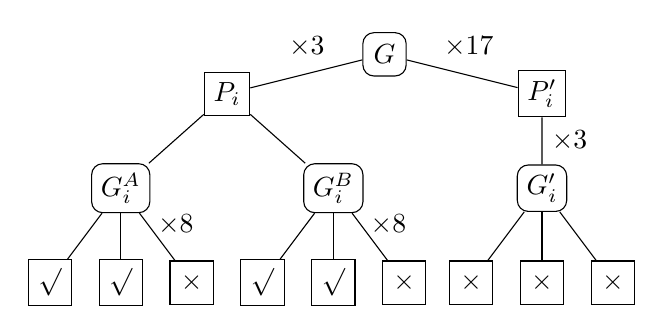
\begin{tikzpicture}[level distance=1.2cm]

\tikzstyle{planbox}=[draw,minimum height=0.55cm,minimum width=0.55cm]
\tikzstyle{goalbox}=[draw,rounded corners,minimum height=0.55cm,minimum width=0.55cm]

\tikzstyle{level 1}=[sibling distance=4cm,level distance=0.5cm] 
\tikzstyle{level 2}=[sibling distance=2.7cm,level distance=1.2cm]
\tikzstyle{level 3}=[sibling distance=.9cm]
\tikzstyle{level 4}=[sibling distance=1cm]

\node[goalbox] (T) {$G$}
   child[solid] {node[planbox] (1) {$P_i$}
      	child {node[goalbox] (11) {$G_i^A$}
			child {node[planbox] {$\surd$}
			}
			child {node[planbox] {$\surd$}
			}
			child {node[planbox] {$\times$}
				edge from parent node[right,near start] {$\times 8$}
			}
	  	}
      	child {node[goalbox] (11) {$G_i^B$}
			child {node[planbox] {$\surd$}
			}
			child {node[planbox] {$\surd$}
			}
			child {node[planbox] {$\times$}
				edge from parent node[right,near start] {$\times 8$}
			}
	  	}
	edge from parent node[above left, near start] {$\times 3$}
   }
   child[solid] {node[planbox] (2) {$P_i'$}
      child {node[goalbox] (22) {$G_i'$} 
	child {node[planbox] {$\times$}}
	child {node[planbox] {$\times$}}
	child {node[planbox] {$\times$}}
	edge from parent node[right] {$\times 3$}
	}
   edge from parent node[above right,near start] {$\times 17$}};

% \draw (T) -- (1) node (aux1) [coordinate,midway]{};
% \draw (T) -- (2) node (aux2) [coordinate,midway]{};
% \draw (aux1) .. controls +(0.3,-0.3) and +(-0.3,-0.3).. (aux2)
% 			node[midway,above] {OR};

% \draw (1) -- (11) node (aux21) [coordinate,midway]{};
% \draw (1) -- (12) node (aux23) [coordinate,midway]{};
% \draw (aux21) .. controls +(0.25,-0.25) and +(-0.25,-0.25).. (aux23)
% 			node[midway,above] {AND};

% \node[below left of=T,text width=2cm,xshift=-3cm] (label)
% 		{$P_i$: plan \\ $G_i$: goals \\ $SG_i$: sub-goals};
\end{tikzpicture}
}

Structure where one of many complex options has a solution. This configuration suits the aggressive \alert{ACL} approach.

\end{frame}

%%%
\begin{frame}{Results: Goal-Plan Structure T1}
\setcounter{framenumber}{\value{finalframe}}

\centering\resizebox{.7\paperwidth}{!}{%!TEX root = ../dsingh-aamas10-poster.tex
\begin{tikzpicture}[x= 0.008cm,y=9cm]
	\definecolor{darkblue}{rgb}{0.1,0.1,0.5}
	\definecolor{darkred}{rgb}{0.8,0.0,0.1}
    % Draw the axes and grid lines
    \draw[-] (0,0) -- (0,1) -- (2000,1) -- (2000,0) -- cycle; 
    \draw[-,thin, dotted, ystep=0.2, xstep=2000] (0,0) grid (2000,1);
    \foreach \x in {500, 1000, 1500}  \draw [-,xshift=0](\x,4pt) -- (\x,-1pt);
    \foreach \y in {0.0,0.2,0.4,0.6,0.8,1.0}  \draw [-,yshift=0](4pt,\y) -- (-1pt,\y);
    \foreach \x/\xtext in {500/500, 1000/1000, 1500/1500} \node at (\x,0) [below] {\xtext};
    \foreach \y/\ytext in {0.0,0.2,0.4,0.6,0.8,1.0}  \node at (0,\y) [left] {\ytext};
    \node at (0,1.15) {Success};
    \node at (1650,0.1) {Iterations};
    \draw[-,darkred] plot[mark=x,mark size=10,mark options={color=darkred}] 
			file {figs/data/test01v3gm.CP.tikzdata};
    \draw[-,darkblue] plot[mark=o,mark size=6,mark options={color=darkblue}] 
			file {figs/data/test01v3gm.SP.tikzdata};
    % Also draw the expected convergence: 0.9^4 actions=0.6561
    \draw[dashed,-,yshift=0](0,0.81) -- (2000,0.81);
	\node at (2300,0.5) {$\mathcal{T}1$};
\end{tikzpicture}
}

Performance of ACL (crosses) vs. BUL (circles). \\Dashed line shows optimal performance.

\end{frame}

%%%
\begin{frame}{Goal-Plan Structure T2}
\setcounter{framenumber}{\value{finalframe}}

\centering\resizebox{.55\paperwidth}{!}{%!TEX root = ../dsingh-aamas10.tex
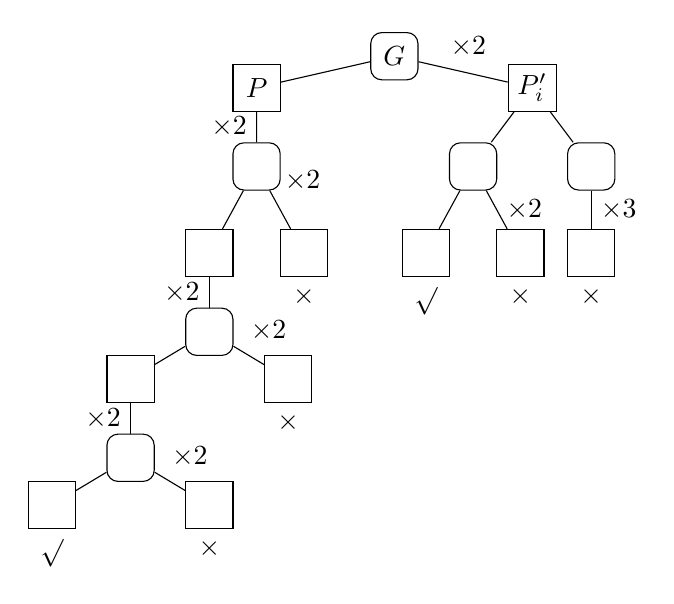
\begin{tikzpicture}[level distance=1.2cm]
\tikzstyle{txt}=[scale=.9]

\tikzstyle{succ}=[label=below:$\surd$]
\tikzstyle{fail}=[label=below:$\times$]


\tikzstyle{planbox}=[draw,minimum height=0.6cm,minimum width=0.6cm]
\tikzstyle{goalbox}=[draw,rounded corners,minimum height=0.6cm,minimum width=0.6cm]

\tikzstyle{level 1}=[sibling distance=3.5cm,level distance=0.4cm] 
\tikzstyle{level 2}=[sibling distance=1.5cm,level distance=1.0cm]
\tikzstyle{level 3}=[sibling distance=1.2cm,level distance=1.1cm]
\tikzstyle{level 4}=[sibling distance=1.2cm,level distance=1.0cm]
\tikzstyle{level 5}=[sibling distance=2.0cm,level distance=0.6cm]
\tikzstyle{level 6}=[sibling distance=1.2cm,level distance=1.0cm]
\tikzstyle{level 7}=[sibling distance=2.0cm,level distance=0.6cm]
\tikzstyle{level 8}=[sibling distance=1.2cm,level distance=1.0cm]

\node[goalbox] (T) {$G$}
   child[solid] {node[planbox] (1) {$P$}
      child {node[goalbox] (11) {\phantom{$G$}}
		child {node[planbox] {\phantom{$P$}}
			child {node[goalbox] {\phantom{$G$}}
				child {node[planbox] {\phantom{$P$}}
					child {node[goalbox] {\phantom{$G$}}
						child {node[planbox,succ] {\phantom{$P$}}}
						child {node[planbox,fail] {\phantom{$P$}}
							edge from parent node[above right,near start] {$\times 2$}
						}
						edge from parent node[left] {$\times 2$}
					}
				}
				child {node[planbox,fail] {$\phantom{P}$}
					edge from parent node[above right,near start] {$\times 2$}
				}
		               edge from parent node[left] {$\times 2$}
			}
		}
		child {node[planbox,fail] {\phantom{$P$}}
			edge from parent node[above right,near start] {$\times 2$}
		}
               edge from parent node[left] {$\times 2$}
	}
   }
   child[solid] {node[planbox] (2) {$P_i'$}
      	child {node[goalbox] (11) {\phantom{$G$}}
			child {node[planbox,succ] {$\phantom{P}$}}
			child {node[planbox,fail] {$\phantom{P}$} 
		               edge from parent node[right] {$\times 2$}
			}
	}
      	child {node[goalbox] {\phantom{$G$}}
			child {node[planbox,fail] {$\phantom{P}$} 
		               edge from parent node[right] {$\times 3$}
			}
	}
	edge from parent node[above right, near start] {$\times 2$}
};
\end{tikzpicture}


}

Structure has solution in one complex option. \\ This configuration suits the conservative \alert{BUL} approach.

\end{frame}

%%%
\begin{frame}{Results: Goal-Plan Structure T2}
\setcounter{framenumber}{\value{finalframe}}

\centering\resizebox{.7\paperwidth}{!}{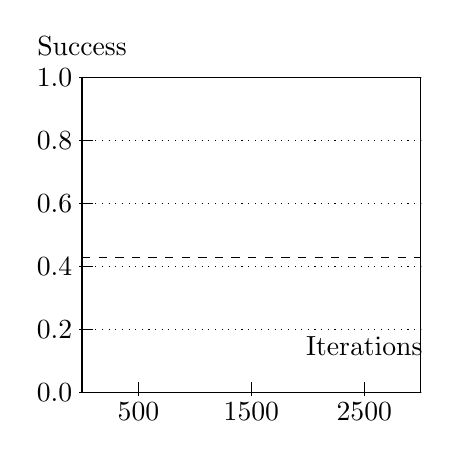
\begin{tikzpicture}[x=0.00143cm,y=4cm]
    % Draw the axes and grid lines
    \draw[-] (0,0) -- (0,1) -- (3000,1) -- (3000,0) -- cycle; 
    \draw[-,thin, dotted, ystep=0.2, xstep=3000] (0,0) grid (3000,1);
    \foreach \x in {500, 1500, 2500}  \draw [-,xshift=0](\x,4pt) -- (\x,-1pt);
    \foreach \y in {0.0,0.2,0.4,0.6,0.8,1.0}  \draw [-,yshift=0](4pt,\y) -- (-1pt,\y);
    \foreach \x/\xtext in {500/500, 1500/1500, 2500/2500} \node at (\x,0) [below] {$\xtext$};
    \foreach \y/\ytext in {0.0,0.2,0.4,0.6,0.8,1.0}  \node at (0,\y) [left] {$\ytext$};
    \node at (0,1.1) {Success};
    \node at (2500,0.15) {Iterations};
    \draw[-] plot[mark=triangle,gray,mark size=3,mark options={color=gray}] 
			file {data/test05v3gm.CP.tikzdata};
    \draw[-] plot[mark=o,gray,mark size=2,mark options={color=gray}] 
			file {data/test05v3gm.SP.tikzdata};
    % Also draw the expected convergence: 0.9^8 actions=0.43046
    \draw[dashed,-,yshift=0](0,0.43046) -- (3000,0.43046);

\end{tikzpicture}
}

Performance of ACL (crosses) vs. BUL (circles). \\Dashed line shows optimal performance.

\end{frame}

%%%
\begin{frame}{Goal-Plan Structure T3}
\setcounter{framenumber}{\value{finalframe}}

\centering\resizebox{.7\paperwidth}{!}{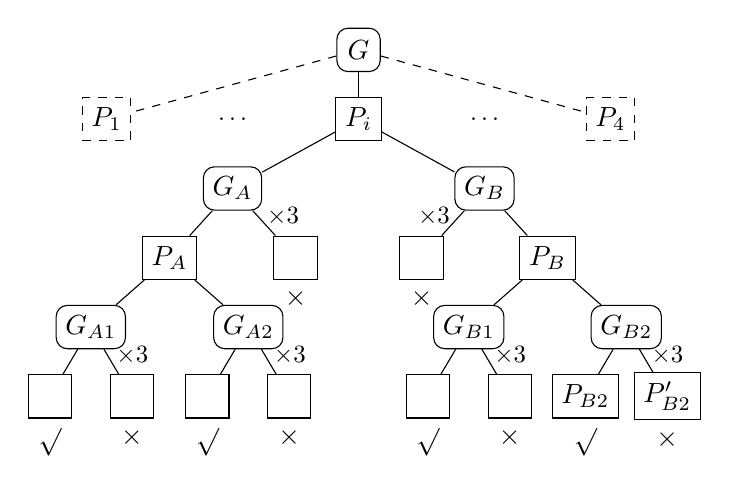
\begin{tikzpicture}[scale=0.8,level distance=1.1cm]
\tikzstyle{txt}=[scale=.9]
\tikzstyle{succ}=[label=below:$\surd$]
\tikzstyle{fail}=[label=below:$\times$]

\tikzstyle{planbox}=[draw,minimum height=0.55cm,minimum width=0.55cm]
\tikzstyle{goalbox}=[draw,rounded corners,minimum height=0.55cm,minimum width=0.55cm]

	
\tikzstyle{level 1}=[sibling distance=4.0cm] 
\tikzstyle{level 2}=[sibling distance=4cm] 
\tikzstyle{level 3}=[sibling distance=2cm]
\tikzstyle{level 4}=[sibling distance=2.5cm]
\tikzstyle{level 5}=[sibling distance=1.3cm]

\node[goalbox,yshift=1cm,solid] (T) {$G$}
	child[dashed] {node[planbox] (P1) {$P_1$}}
	child[solid] {node[planbox] (Pi) {$P_i$}
		child {node[goalbox] {$G_A$}
			child {node[planbox] {$P_{A}$}
				child {node[goalbox] {$G_{A1}$}
					child {node[planbox,succ] {$\phantom{P}$}}
					child {node[planbox,fail] {$\phantom{P}$} 
					edge from parent node[txt,right,near start] {$\times 3$}
					}
				}
				child {node[goalbox] {$G_{A2}$}
					child {node[planbox,succ] {$\phantom{P}$}}
					child {node[planbox,fail] {$\phantom{P}$} 
						edge from parent node[txt,right,near start] {$\times 3$}
					}
				}
			}
			child {node[planbox,fail] {$\phantom{P}$} 
				edge from parent node[txt,right,near start] {$\times 3$}
			}
		}
		child {node[goalbox] {$G_{B}$}
			child {node[planbox,fail] {$\phantom{P}$}
				edge from parent node[txt,left,near start] {$\times 3$}
			}
			child {node[planbox] {$P_B$}
				child {node[goalbox] {$G_{B1}$}
					child {node[planbox,succ] {$\phantom{P}$}}
					child {node[planbox,fail] {$\phantom{P}$}
						edge from parent node[txt,right,near start] {$\times 3$}
					}
				}
				child {node[goalbox] {$G_{B2}$}
					child {node[planbox,succ] {$P_{B2}$}}
					child {node[planbox,fail] {$P_{B2}'$}
						edge from parent node[txt,right,near start] {$\times 3$}
					}
				}
			}
		}
	}
	child[dashed] {node[planbox] (P4) {$P_4$}}
;
\node[txt] at ($ (P1)!.5!(Pi) $) {$\ldots$};
\node[txt] at ($ (Pi)!.5!(P4) $) {$\ldots$};

\end{tikzpicture}
}

Structure where both schemes show \alert{comparable performance}.

\end{frame}

%%%
\begin{frame}{Results: Goal-Plan Structure T3}
\setcounter{framenumber}{\value{finalframe}}

\centering\resizebox{.7\paperwidth}{!}{%!TEX root = ../dsingh-aamas10-poster.tex
\begin{tikzpicture}[x=0.0032cm,y=9cm]
    % Draw the axes and grid lines
    \draw[-] (0,0) -- (0,1) -- (5000,1) -- (5000,0) -- cycle; 
    \draw[-,thin, dotted, ystep=0.2, xstep=5000] (0,0) grid (5000,1);
    \foreach \x in {1000, 2500, 4000}  \draw [-,xshift=0](\x,4pt) -- (\x,-1pt);
    \foreach \y in {0.0,0.2,0.4,0.6,0.8,1.0}  \draw [-,yshift=0](4pt,\y) -- (-1pt,\y);
    \foreach \x/\xtext in {1000/1000, 2500/2500, 4000/4000} \node at (\x,0) [below] {\xtext};
    \foreach \y/\ytext in {0.0,0.2,0.4,0.6,0.8,1.0}  \node at (0,\y) [left] {\ytext};
    \node at (0,1.15) {Success};
    \node at (4150,0.1) {Iterations};
    \draw[-,red] plot[mark=x,mark size=10,mark options={color=red}] 
			file {figs/data/testImpactvars2.CP.tikzdata};
    \draw[-,blue] plot[mark=o,mark size=6,mark options={color=blue}] 
			file {figs/data/testImpactvars2.SP.tikzdata};
    % Also draw the expected convergence: 0.9^4 actions=0.6561
    \draw[dashed,-,yshift=0](0,0.6561) -- (5000,0.6561);
	\node at (5700,0.5) {$\mathcal{T}3$};

\end{tikzpicture}
}

Performance of ACL (crosses) vs. BUL (circles). \\Dashed line shows optimal performance.

\end{frame}


\end{document}
%%%
